\section{Mechatronics}
\label{sec:mechatronics}
This section specifies the components used for the solar panel drive mechanism. The implementation of hardware redundancy is considered during the design phase, since the system's fault tolerance is a driving aspect of this project. This redundancy is represented in the choice and quantity of specific components. Table \ref{tab:component_list} displays all the components, their quantities and corresponding details.

\subsection{Microcontroller}
This system uses an Arduino Mega 2560 microcontroller. Arduino offers not only boards containing the processor, memory, I/Os, and power system in a compact interface but also allows for easy software integration. To fulfil the requirement of fault tolerance, this system has a second microcontroller of the same kind in a watchdog configuration. Once the master microcontroller fails to reset the watchdog's timer, the second (slave) microcontroller takes over, in case the latter cannot reset the master board. This configuration uses an Arduino Mega 2560 instead of the Arduino Uno, due to the increased amount of pins available, which are required for the system to function properly, regarding the fault tolerance.

\subsection{Rotation mechanism}
To move the solar panel into the assigned angular position a motor is needed. For this project, an uni-polar stepper motor is used as the system's actuator. The idea is that the motor drives an axis on which the solar panel sits,  which is then rotated into the defined position. The motor rotates in fixed angular increments, instead of moving continuously, which makes stepper motors very precise and suitable for the application in a solar panel drive mechanism. Another advantage of the stepper motor is its capacity to hold torque also when it is not powered. The 28BYJ-48 stepper motor is used for the driving mechanism and integrated into the system setup through its the ULN2003 driver board. The other end of the rotation axis holds the potentiometer used to verify the angular position obtained by the stepper motor. Here, a concerning challenge is the reproducibility of the potentiometer feedback since its linear output has a standard tolerance of 20\% \cite{poti}. Figure \autoref{fig:components_rotation} depicts the stepper motor and its driver board, and the potentiometer.

\begin{figure}[H]
    \centering
    \begin{subfigure}[b]{0.3\textwidth}
       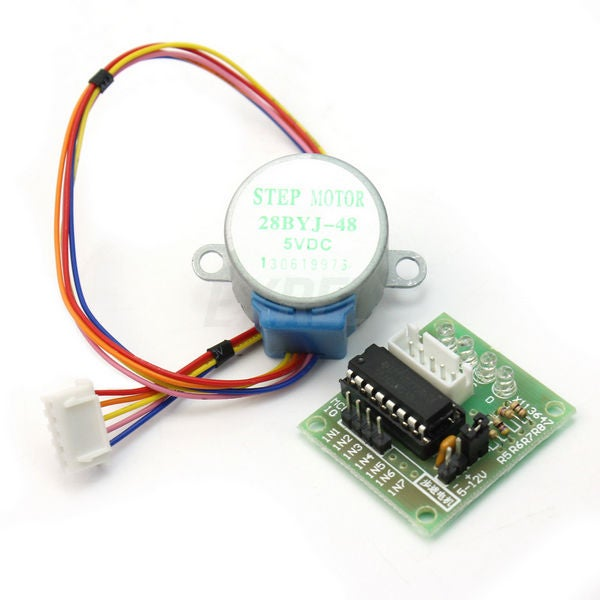
\includegraphics[width=\textwidth]{figures/steppermotor_board.jpg}
       \caption{28BYJ-48 stepper motor and ULN2003 driver board}
    \end{subfigure}
    \begin{subfigure}[b]{0.3\textwidth}
       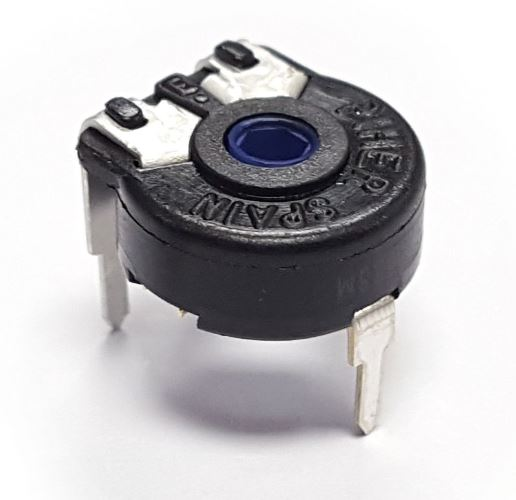
\includegraphics[width=\textwidth]{figures/pot.JPG}
       \caption{Piher PT10 potentiometer}
    \end{subfigure}
    \caption{Solar panel mounting structure}
    \label{fig:components_rotation}
\end{figure}{}


\subsection{Visual feedback}
Besides the serial monitor, the user receives visual feedback about the state of the system through a set of LEDs and an LCD screen. The former provides information regarding the operation status of the stepper motor. The latter shows the current angle of the solar panel and additional information about the system.

\subsection{Other components}
Two breadboards are part of the system setup accommodating the LEDs, LCD, and necessary jumper wires. The majority of wires are in male/male configuration, while male/female jumper wires connect the potentiometers and motor driver boards. Additionally, $\unit[220]{\Omega}$ resistors adjust the current flowing to the visual components.



\begin{table}[H]
    \centering
    \begin{tabular}{|l|r|c|}
        \hline
        Component   &  Quantity &  Details\\ \hline
        Microcontroller  & 2     & Arduino Mega 2560 plus USB cable\\
        Stepper motor & 2 & 28BYJ-48\\
        Stepper motor driver & 2 & ULN2003 driver board\\
        Potentiometer & 3 & Piher PT10 50K\\
        LCD screen & 1 & NDS1602A module\\
        LED (red \& green) & 4 &  --\\
        Resistor & 5 & 220 Ohm\\
        Breadboard & 2 & --\\
        Jumper wires & 30+ & male/male \& male/female \\
        \hline
    \end{tabular}
    \caption{List of components}
    \label{tab:component_list}
\end{table}{}